%preamble
\documentclass[12pt,a4paper]{article}

%inputs for firstpage
\def \CourseName {گزارش فاز سوم}
\def \Instructor {دکتر مسلم حبیبی}
\def \Semester {نیم‌سال دوم\\سال تحصیلی 99-00}


%packages
\usepackage[]{algorithm2e}
\usepackage{cite}
\usepackage{calc}
\usepackage{fancyhdr}
\usepackage{lipsum}
\usepackage{color}
\usepackage{ragged2e}
\usepackage[inline]{enumitem}
\usepackage[dvipsnames]{xcolor}
\usepackage{graphicx}
\usepackage{wrapfig}
\usepackage{float}
\usepackage[skip=12pt,indent=2em]{parskip}
\usepackage{setspace}
\usepackage{textcomp}
\usepackage{etoolbox}
\usepackage{xpatch}
\usepackage{tabu}
\usepackage{hyperref}


%for persian fonts
\usepackage{xepersian}
\defpersianfont\bnazanin{BNazanin}
\settextfont{BNazanin}

\title{
	\center
	
\includegraphics[width=5cm, height=5cm]{images/shariflogo.jpg} \\
	دانشکده مهندسی صنایع \\
	دانشگاه صنعتی شریف \\
	\CourseName
}
\author{
	\\
	\\
	\textbf{استاد درس:}
	\\
	\Instructor \\[35pt]
	\\
	\textbf{نام اعضای گروه:}
	\\مهدی محسنی 
	\\محراب کشاورز گیلده 
	\\احسان چشمی
	\\[45pt]
}
\date{{\small\Semester}}



%body
\begin{document}

\maketitle
\pagebreak
\tableofcontents
\pagebreak
\listoffigures
\pagebreak
\normalsize	



\pagebreak
\section{رسم فرایندها} \label{section.function}

\textbf{نکته:}
برای گرفتن خروجی به فرمت \lr{image} در نرم افزار بیزاجی مشکلی که وجود دارد این است که حروف فارسی را به خوبی پشتیبانی نمی کند و در نتیجه کلمات جا به جا شده و برعکس نشان داده می شوند.


خروجی \lr{pdf} و \lr{microsoft word}نیز مشکل دارد و با ارور زیر مواجه می شود:
	\begin{figure}[h!]
	\begin{center}
		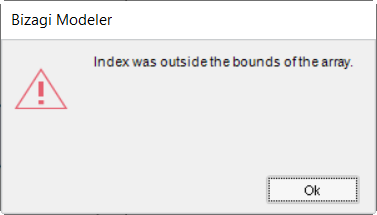
\includegraphics[width=10cm]{images/Error.png}	
	\end{center}
	\caption{پیام خطا}
	\end{figure}


به همین علت به صورت اسکرین شات عکس های پروژه را در گزارش آورده ایم.


تنها خروجی ممکن خروجی به ویزیو بوده است که آن را نیز در فایل \lr{zip} "خروجی های بیزاجی" پروژه آورده ایم.
\pagebreak

\subsection{فرایند ثبت نام} \label{section.function.register}
	
	\begin{figure}[h!]
		\begin{center}
			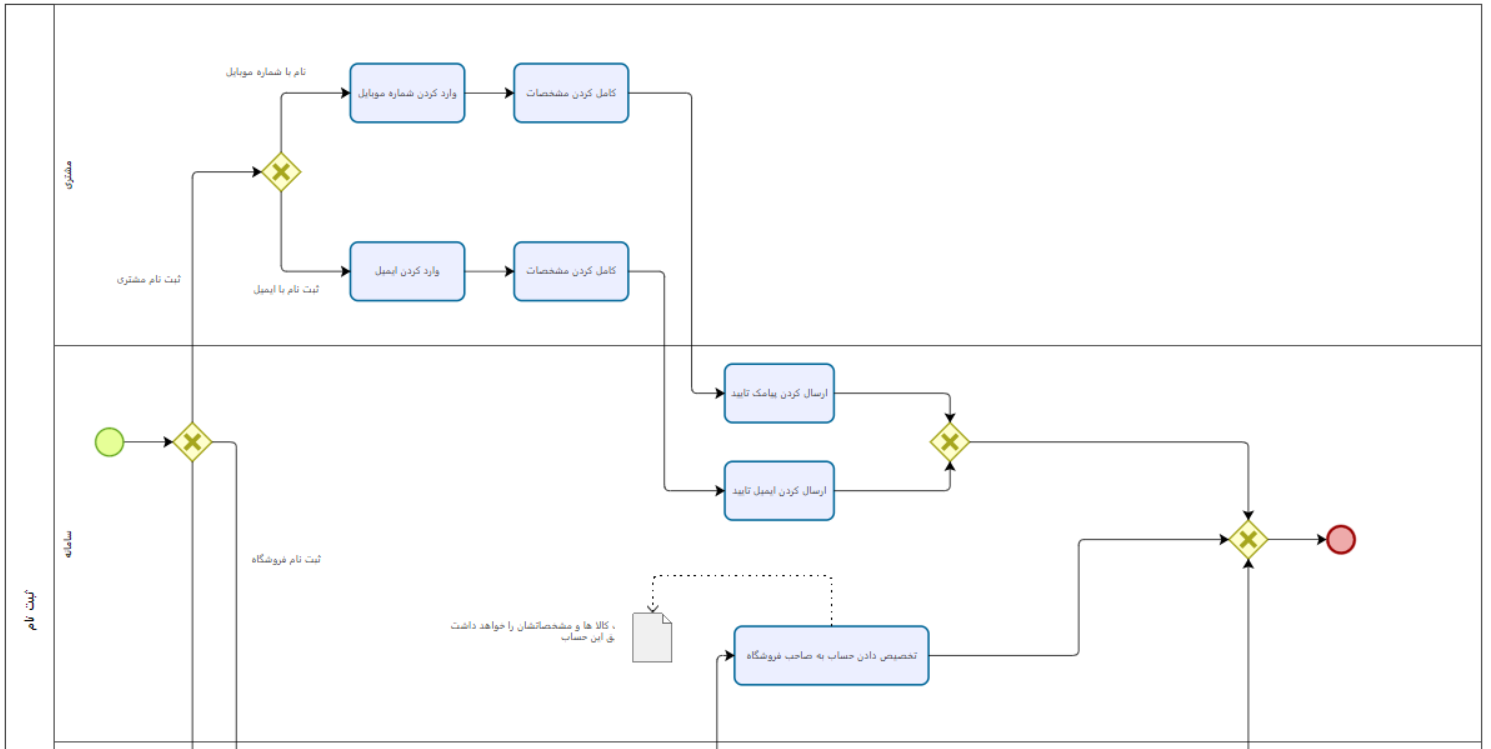
\includegraphics[width=14cm]{images/Bizagi Register 1.png}	
		\end{center}
		\caption{ثبت نام - 1}
	\end{figure}
	\begin{figure}[h!]
		\begin{center}
			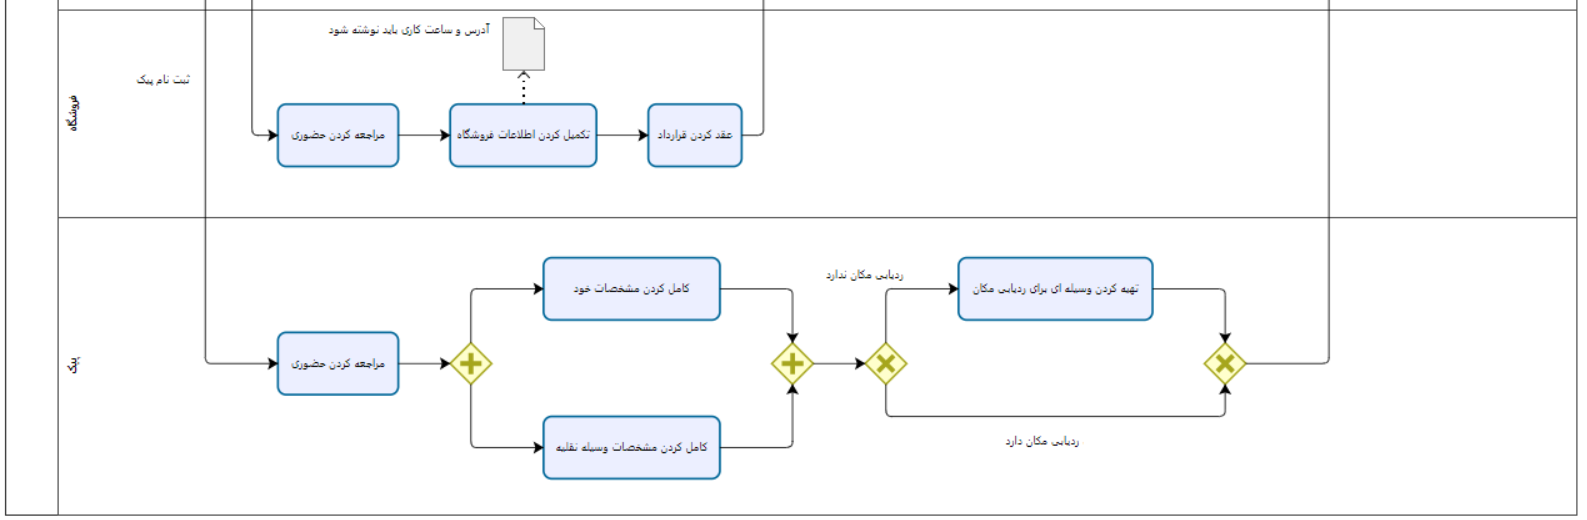
\includegraphics[width=14cm]{images/Bizagi Register 2.png}	
		\end{center}
		\caption{ثبت نام - 2}
	\end{figure}
	
	\textbf{توضیحات}
	
	
	\pagebreak

\subsection{فرایند خرید} \label{section.function.buy}
	\begin{figure}[h!]
		\begin{center}
			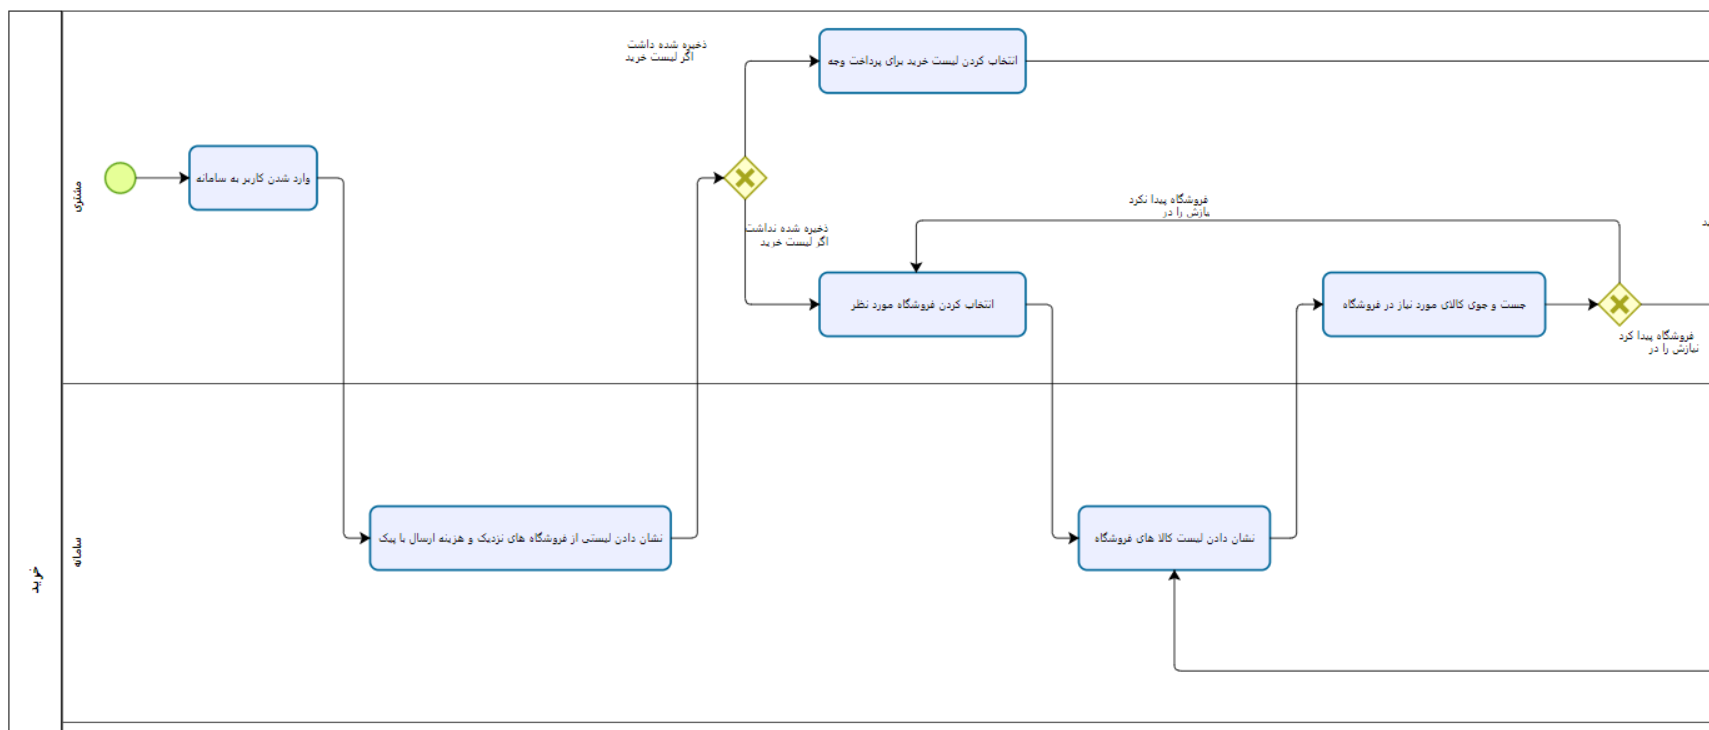
\includegraphics[width=14cm]{images/Bizagi Buy 1.png}	
		\end{center}
		\caption{خرید - 1}
	\end{figure}
	\begin{figure}[h!]
		\begin{center}
			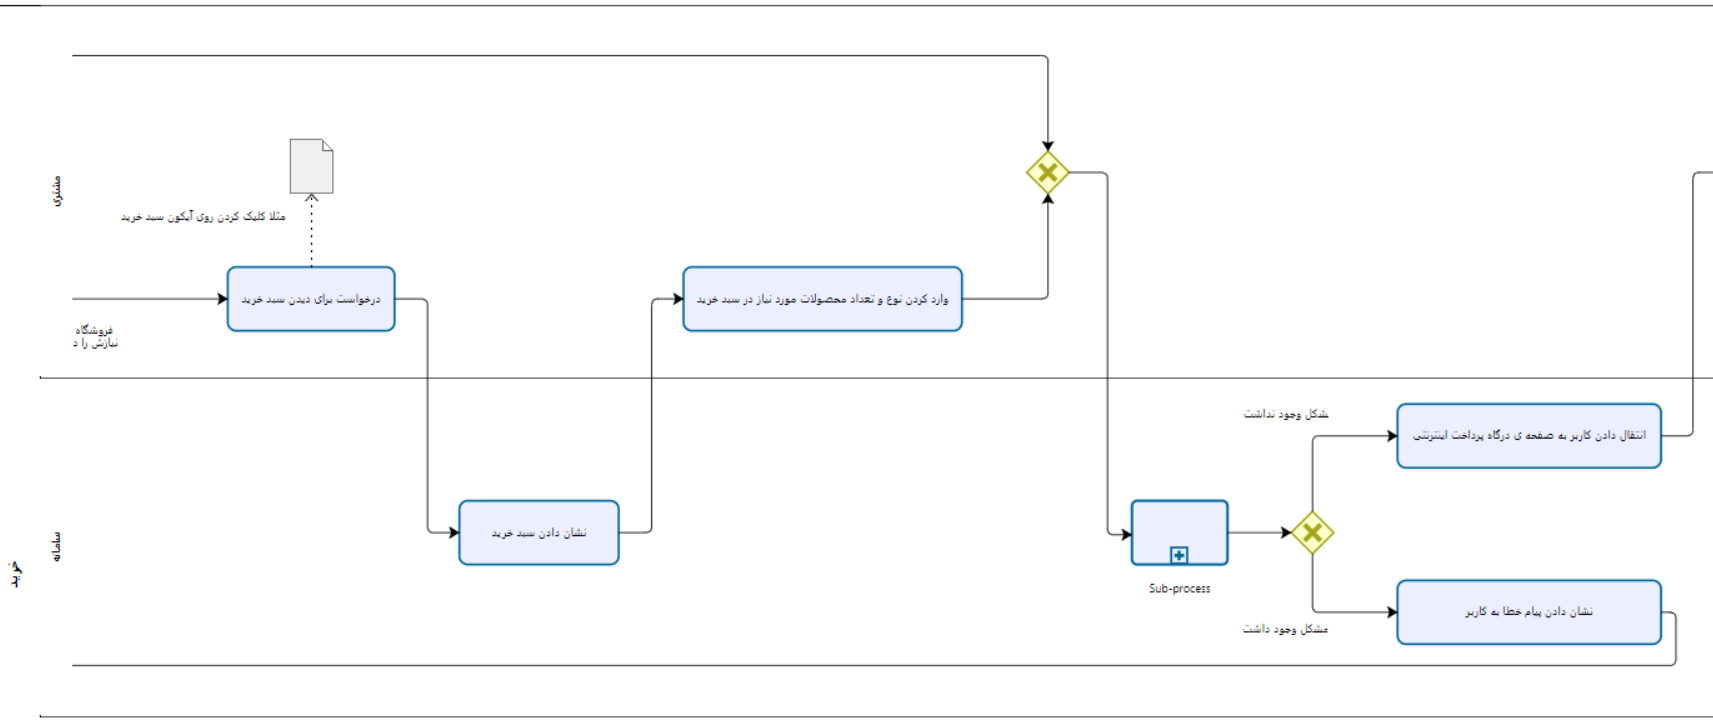
\includegraphics[width=14cm]{images/Bizagi Buy 2.png}	
		\end{center}
		\caption{خرید - 2}
	\end{figure}
	\pagebreak
	\begin{figure}[h!]
		\begin{center}
			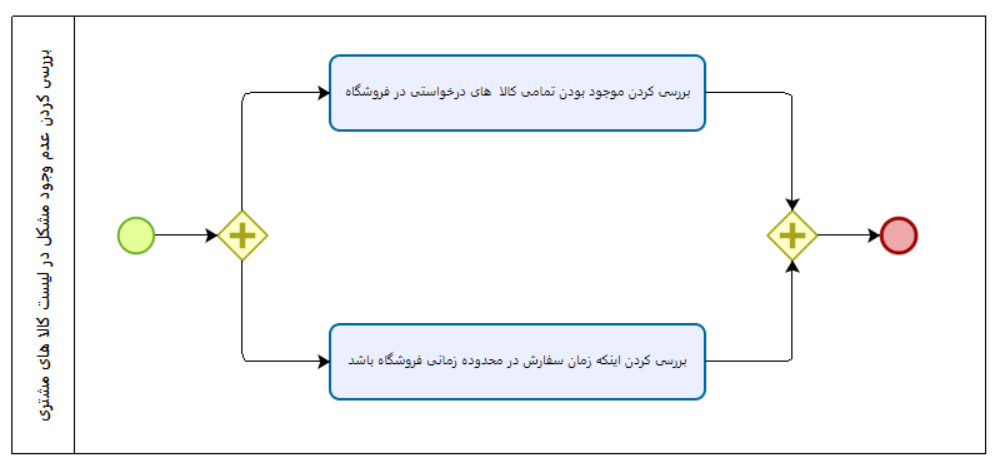
\includegraphics[width=14cm]{images/Bizagi Buy Sub-Process.png}	
		\end{center}
		\caption{خرید - \lr{sub-process}}
	\end{figure}
	\begin{figure}[h!]
		\begin{center}
			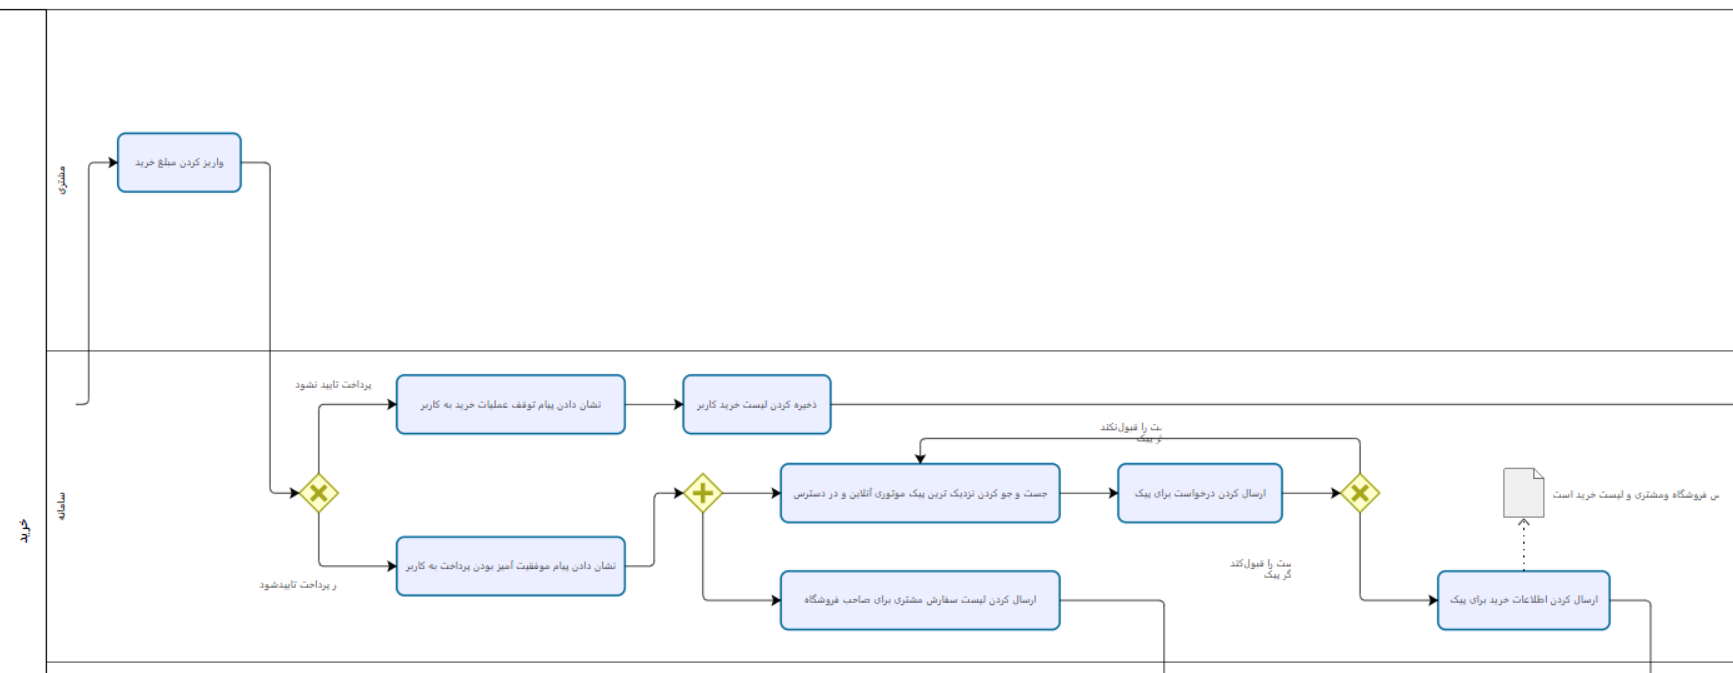
\includegraphics[width=14cm]{images/Bizagi Buy 3.png}	
		\end{center}
		\caption{خرید - 3}
	\end{figure}
	\begin{figure}[h!]
		\begin{center}
			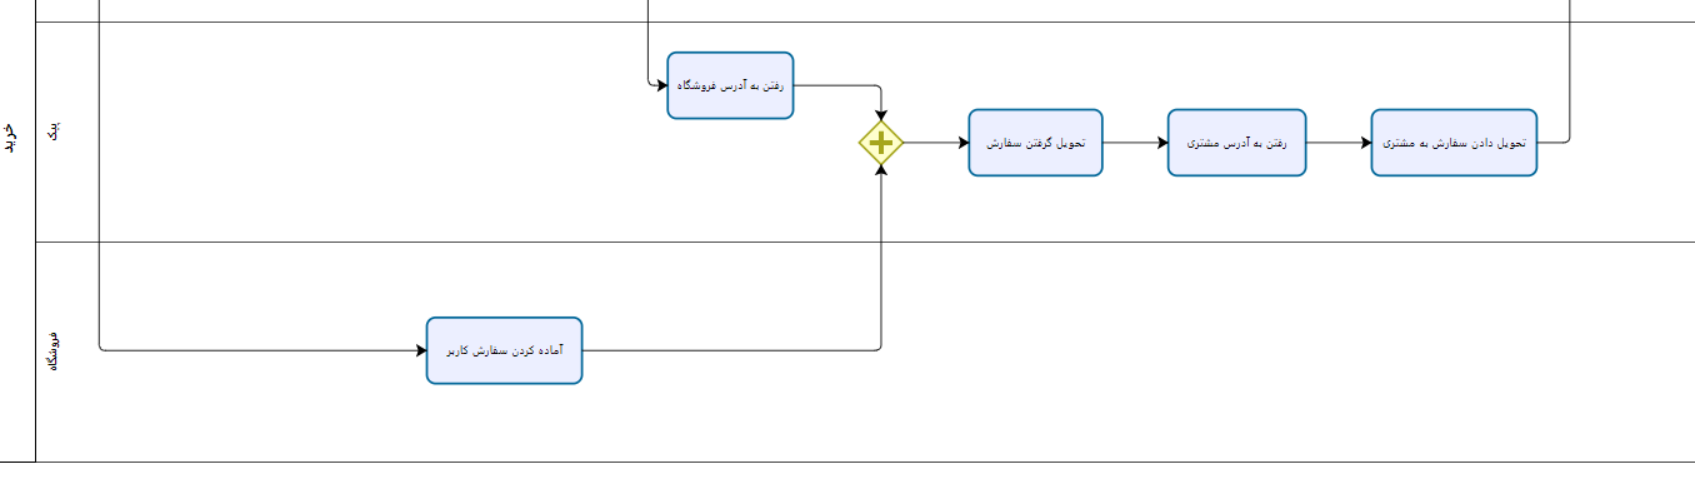
\includegraphics[width=14cm]{images/Bizagi Buy 4.png}	
		\end{center}
		\caption{خرید - 4}
	\end{figure}
	\pagebreak
	\begin{figure}[h!]
		\begin{center}
			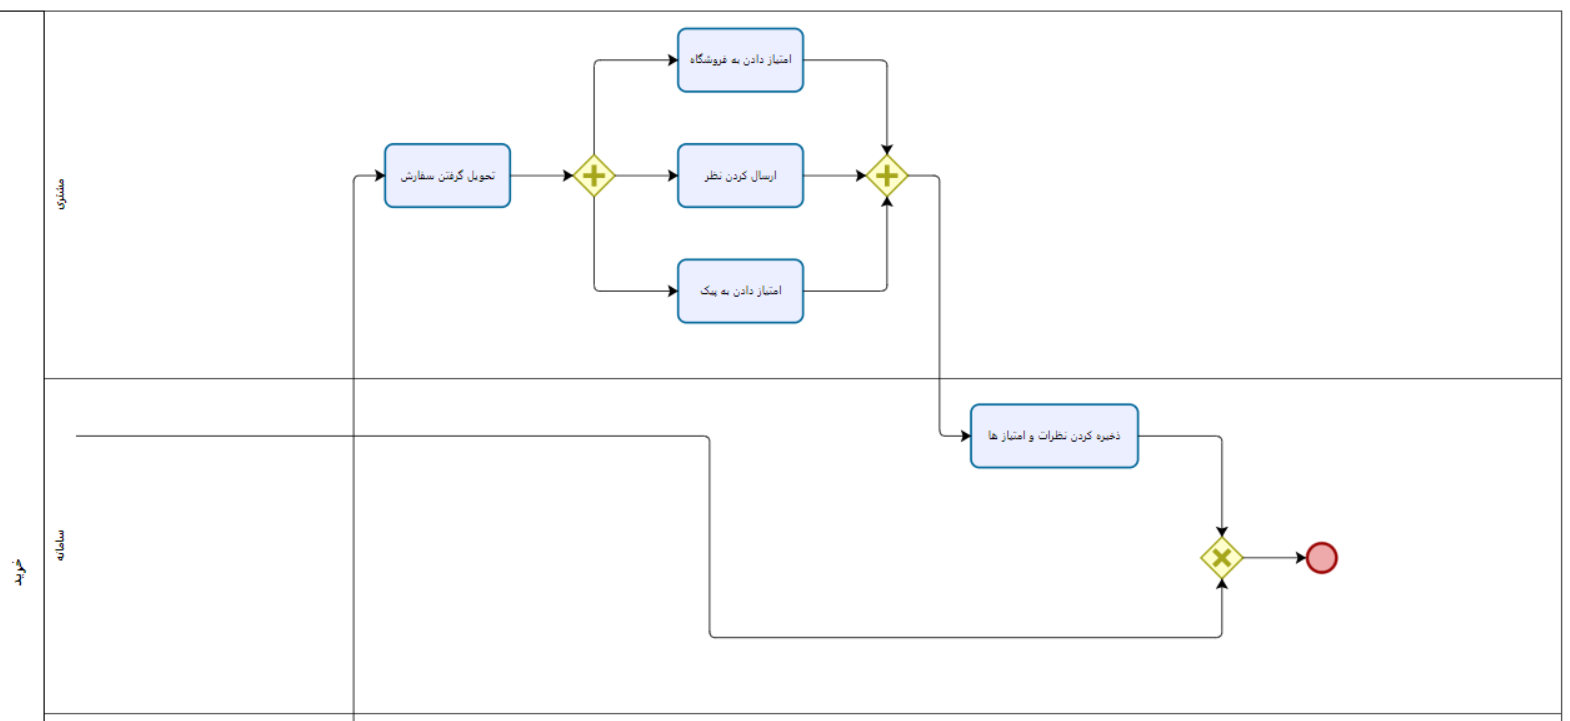
\includegraphics[width=14cm]{images/Bizagi Buy 5.png}	
		\end{center}
		\caption{خرید - 5}
	\end{figure}
	
	\textbf{توضیحات}
	
	
	\pagebreak
\subsection{فرایند مرجوعی} \label{section.function.return}

	\begin{figure}[h!]
	\begin{center}
		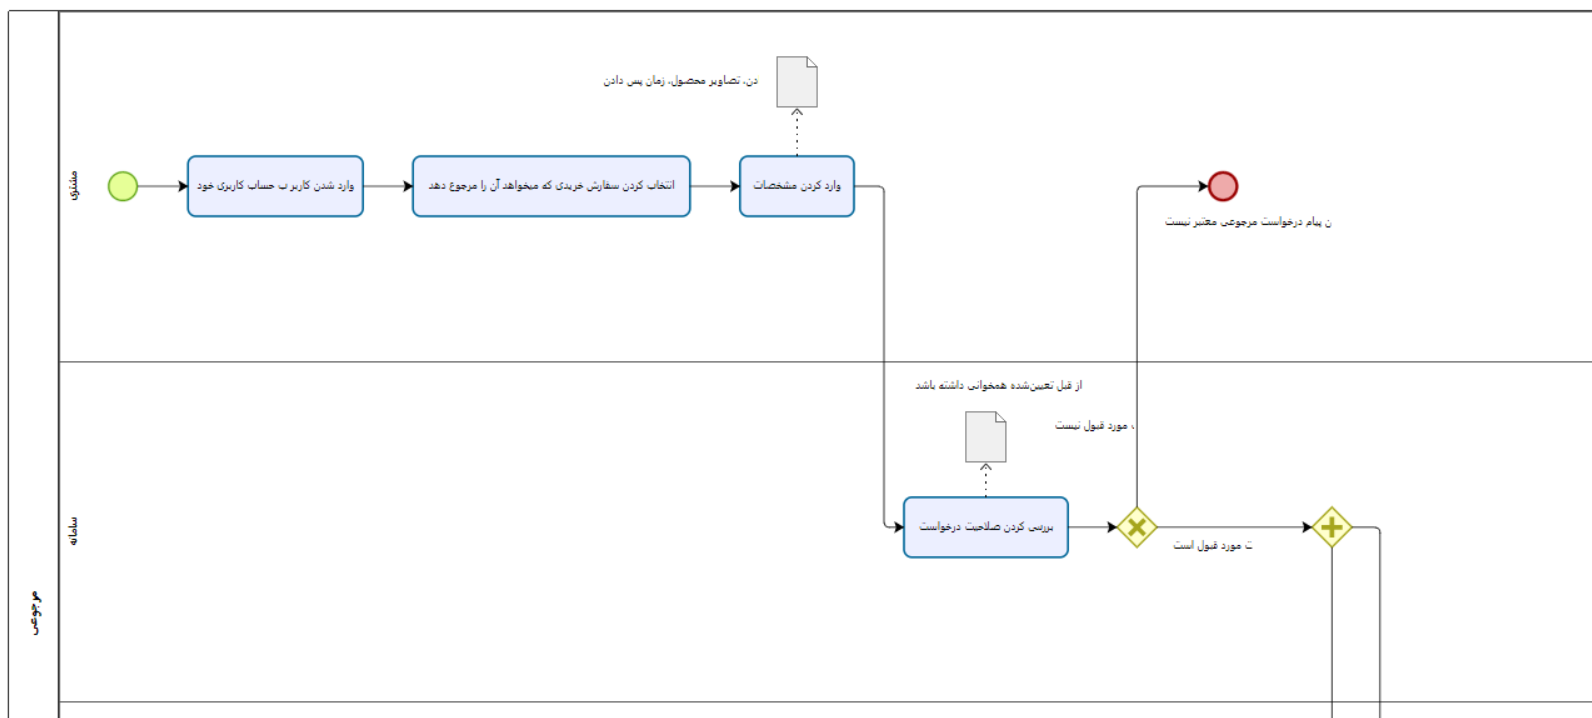
\includegraphics[width=14cm]{images/Bizagi Return 1.png}	
	\end{center}
	\caption{مرجوعی - 1}
\end{figure}
\begin{figure}[h!]
	\begin{center}
		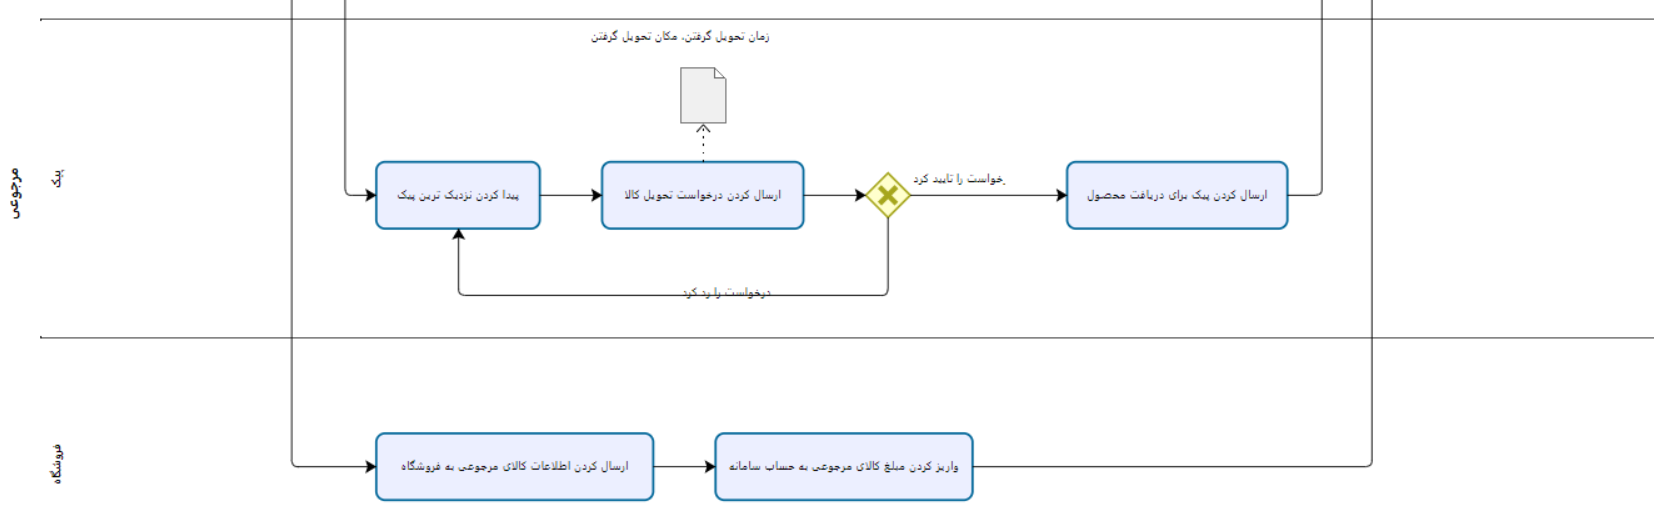
\includegraphics[width=14cm]{images/Bizagi Return 2.png}	
	\end{center}
	\caption{مرجوعی - 2}
\end{figure}
\pagebreak
\begin{figure}[h!]
	\begin{center}
		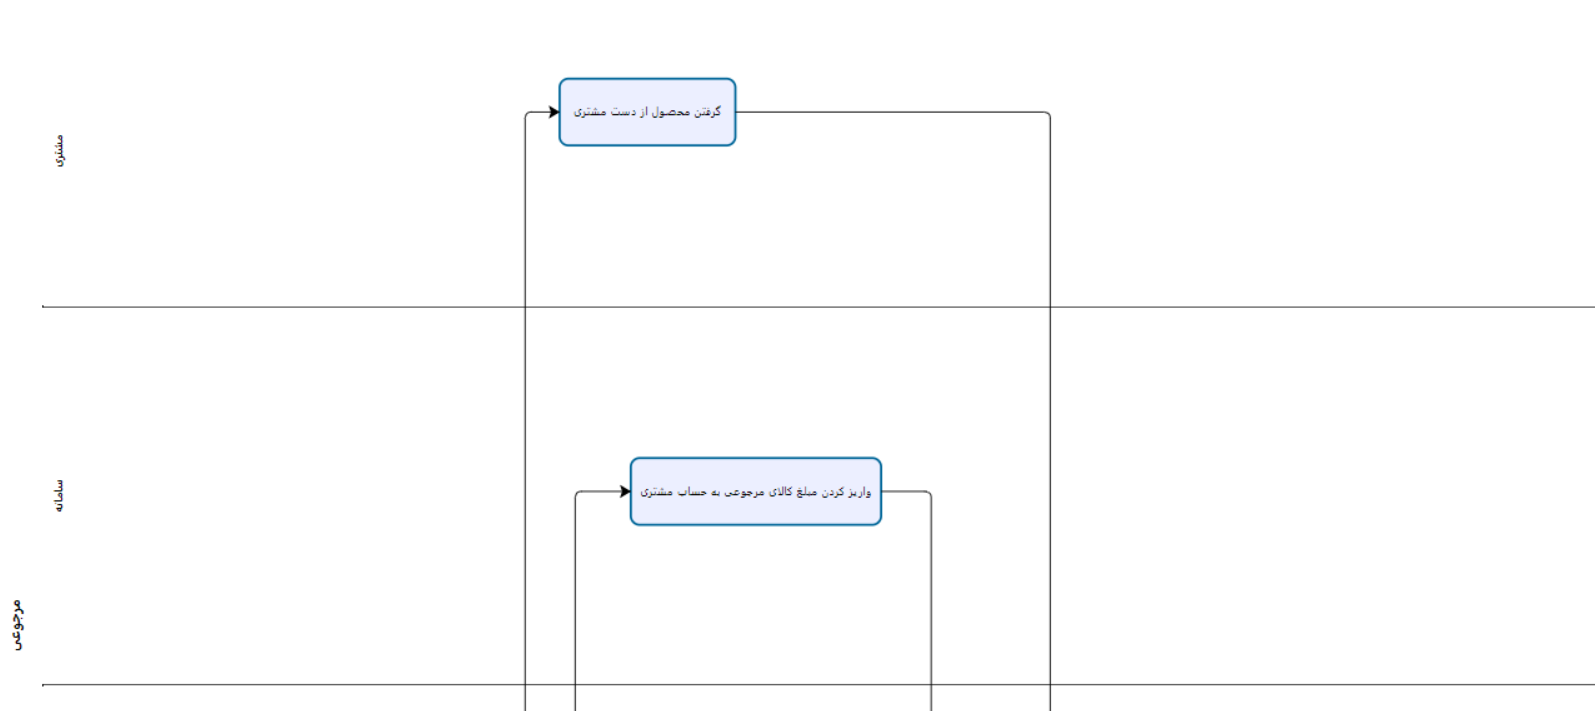
\includegraphics[width=14cm]{images/Bizagi Return 3.png}	
	\end{center}
	\caption{مرجوعی - 3}
\end{figure}
\begin{figure}[h!]
	\begin{center}
		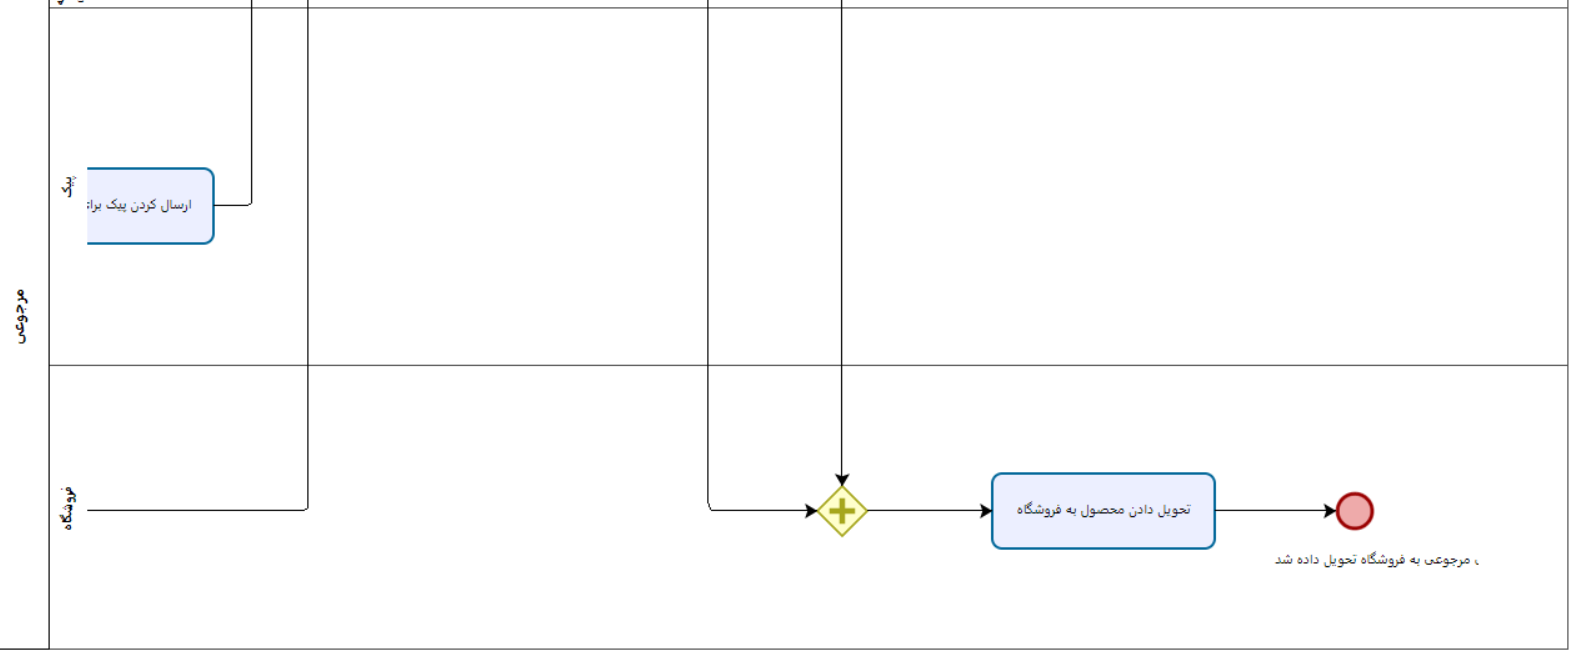
\includegraphics[width=14cm]{images/Bizagi Return 4.png}	
	\end{center}
	\caption{مرجوعی - 4}
\end{figure}

\textbf{توضیحات}


در ابتدا مشتری وارد حساب کاربری خودش می شود. لیست خریدی که داشته را انتخاب می کند. کالایی را که می خواهد مرجوع بزند انتخاب می کند. مشخصات کالا، دلایل پس دادن آن و اطلاعات زمانی و مکانی پس دادن کالا را مشخص می کند. در صورت عدم موافقت با درخواست و نداشتن شرایط لازم برای پس دادن کالا درخواست رد می شود. در صورت موافقت سامانه به دنبال نزدیک ترین پیک می رود و همچنین اطلاعات کالای مرجوعی را به صاحب فروشگاهی که محصول را فروخته بود می دهد. نزدیک ترین پیک که پیدا شد مشخصات کالای مرجوعی برای او ارسال می شود در صورت عدم موافقت او سامانه به دنبال نزدیک ترین پیک بعدی می رود. در صورت موافقت پیک به مکان مورد نظر مشتری در زمان تعیین شده از قبل می رود تا کالای مرجوعی را تحویل گیرد. فروشگاه مبلغ کالای مرجوعی را برای حساب سامانه واریز می کند. سامانه پول دریافتی را برای حساب مشتری واریز می کند. پس از اتمام واریز پول و رفتن پیک و تحویل کالای مرجوعی آن کالای مرجوعی به فروشگاه برگردانده می شود.

\pagebreak

\section{گزارش نحوه انجام پروژه} \label{section.report}
یک روز بعد از اتمام فاز اول جلسه ی پس از مرگ \footnote{\lr{post mortem}} در محیط اسکایپ \footnote{\lr{Skype}}انجام شد و پس از آن جلسه و باتوجه به نتایج بدست آمده از آن، اعضای گروه تصمیم گرفتند که کل این فاز را همگی با هم و در یک مرحله رسم کنند. به این ترتیب که \underline{محراب کشاورز گیلده} نرم افزار بیزاجی\footnote{\lr{Bizagi}} را نصب کند و پس از آن هر سه نمودار در یک روز در یک جلسه سه نفره کشیده شود. روزی که قرار به کشیدن فرایندها شد متاسفانه نرم افزار بسیار مشکل داشت و ما هر چه کردیم نتوانستیم که فایل خود را ذخیره کنیم به همین دلیل مجبور شدیم که فرایندها را در نرم افزار ویزیو\footnote{\lr{Visio}} رسم کنیم. بعد از این که مشکل نرم افزار اصلی برطرف شد، \underline{محراب کشاورز گیلده} فرایندهای رسم شده در ویزیو را در بیزاجی کشید و خروجی های مورد نیاز را گرفت. بعد از آن گزارش لاتک نیز نوشته شده و در جلسه ای با حضور همه ی اعضا، فایل مربوطه برای ارسال آماده شد و در کوئرا\footnote{\lr{https://quera.ir/}} بارگذاری شد.


\textbf{نکته :} متاسفانه در این فاز نیز مانند فاز قبل اعضای گروه به \lr{commit} و \lr{push} کردن مطالب اکتفا کردند و فراموش کردند که مشکلی\footnote{\lr{issue}} که به آن ها اختصاص داده شده بود را بعد از انجام دادن ببندند به همین دلیل تمامی مشکلات در گیت هاب توسط \underline{مهدی محسنی} و در یک زمان بسته شد اما این موضوع به این معنی نیست که همه ی آن ها در یک روز انجام شده باشد. این مطلب حتی در جلسه ی پس از مرگ نیز ذکر شد اما باز هم اعضای گروه فراموش کردند.
\pagebreak

\subsection{\lr{Task board and Burndown Chart}} \label{section.report.taskBoard}

\begin{figure}[h!]
	\begin{center}
		\includegraphics[width=14cm]{images/screenshot_7.png}	
	\end{center}
	\caption{ابتدای اسپرینت}
\end{figure}

\begin{figure}[h!]
	\begin{center}
		\includegraphics[width=14cm]{images/screenshot_1.png}
	\end{center}
	\caption{انتهای اسپرینت}
\end{figure}


%\begin{figure}[h!]
%	\begin{center}
%		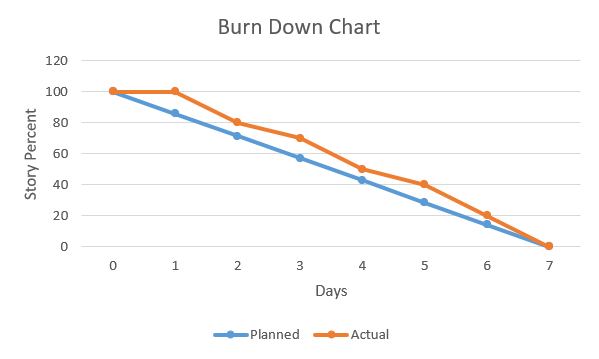
\includegraphics[width=14cm]{images/Burn Down Chart.png}
		
%	\end{center}
%	\caption{\lr{Burn Down Chart}}
%\end{figure}




\end{document}